% Options for packages loaded elsewhere
\PassOptionsToPackage{unicode}{hyperref}
\PassOptionsToPackage{hyphens}{url}
\PassOptionsToPackage{dvipsnames,svgnames,x11names}{xcolor}
%
\documentclass[
  letterpaper,
  DIV=11,
  numbers=noendperiod]{scrartcl}

\usepackage{amsmath,amssymb}
\usepackage{iftex}
\ifPDFTeX
  \usepackage[T1]{fontenc}
  \usepackage[utf8]{inputenc}
  \usepackage{textcomp} % provide euro and other symbols
\else % if luatex or xetex
  \usepackage{unicode-math}
  \defaultfontfeatures{Scale=MatchLowercase}
  \defaultfontfeatures[\rmfamily]{Ligatures=TeX,Scale=1}
\fi
\usepackage{lmodern}
\ifPDFTeX\else  
    % xetex/luatex font selection
\fi
% Use upquote if available, for straight quotes in verbatim environments
\IfFileExists{upquote.sty}{\usepackage{upquote}}{}
\IfFileExists{microtype.sty}{% use microtype if available
  \usepackage[]{microtype}
  \UseMicrotypeSet[protrusion]{basicmath} % disable protrusion for tt fonts
}{}
\makeatletter
\@ifundefined{KOMAClassName}{% if non-KOMA class
  \IfFileExists{parskip.sty}{%
    \usepackage{parskip}
  }{% else
    \setlength{\parindent}{0pt}
    \setlength{\parskip}{6pt plus 2pt minus 1pt}}
}{% if KOMA class
  \KOMAoptions{parskip=half}}
\makeatother
\usepackage{xcolor}
\setlength{\emergencystretch}{3em} % prevent overfull lines
\setcounter{secnumdepth}{-\maxdimen} % remove section numbering
% Make \paragraph and \subparagraph free-standing
\ifx\paragraph\undefined\else
  \let\oldparagraph\paragraph
  \renewcommand{\paragraph}[1]{\oldparagraph{#1}\mbox{}}
\fi
\ifx\subparagraph\undefined\else
  \let\oldsubparagraph\subparagraph
  \renewcommand{\subparagraph}[1]{\oldsubparagraph{#1}\mbox{}}
\fi

\usepackage{color}
\usepackage{fancyvrb}
\newcommand{\VerbBar}{|}
\newcommand{\VERB}{\Verb[commandchars=\\\{\}]}
\DefineVerbatimEnvironment{Highlighting}{Verbatim}{commandchars=\\\{\}}
% Add ',fontsize=\small' for more characters per line
\usepackage{framed}
\definecolor{shadecolor}{RGB}{241,243,245}
\newenvironment{Shaded}{\begin{snugshade}}{\end{snugshade}}
\newcommand{\AlertTok}[1]{\textcolor[rgb]{0.68,0.00,0.00}{#1}}
\newcommand{\AnnotationTok}[1]{\textcolor[rgb]{0.37,0.37,0.37}{#1}}
\newcommand{\AttributeTok}[1]{\textcolor[rgb]{0.40,0.45,0.13}{#1}}
\newcommand{\BaseNTok}[1]{\textcolor[rgb]{0.68,0.00,0.00}{#1}}
\newcommand{\BuiltInTok}[1]{\textcolor[rgb]{0.00,0.23,0.31}{#1}}
\newcommand{\CharTok}[1]{\textcolor[rgb]{0.13,0.47,0.30}{#1}}
\newcommand{\CommentTok}[1]{\textcolor[rgb]{0.37,0.37,0.37}{#1}}
\newcommand{\CommentVarTok}[1]{\textcolor[rgb]{0.37,0.37,0.37}{\textit{#1}}}
\newcommand{\ConstantTok}[1]{\textcolor[rgb]{0.56,0.35,0.01}{#1}}
\newcommand{\ControlFlowTok}[1]{\textcolor[rgb]{0.00,0.23,0.31}{#1}}
\newcommand{\DataTypeTok}[1]{\textcolor[rgb]{0.68,0.00,0.00}{#1}}
\newcommand{\DecValTok}[1]{\textcolor[rgb]{0.68,0.00,0.00}{#1}}
\newcommand{\DocumentationTok}[1]{\textcolor[rgb]{0.37,0.37,0.37}{\textit{#1}}}
\newcommand{\ErrorTok}[1]{\textcolor[rgb]{0.68,0.00,0.00}{#1}}
\newcommand{\ExtensionTok}[1]{\textcolor[rgb]{0.00,0.23,0.31}{#1}}
\newcommand{\FloatTok}[1]{\textcolor[rgb]{0.68,0.00,0.00}{#1}}
\newcommand{\FunctionTok}[1]{\textcolor[rgb]{0.28,0.35,0.67}{#1}}
\newcommand{\ImportTok}[1]{\textcolor[rgb]{0.00,0.46,0.62}{#1}}
\newcommand{\InformationTok}[1]{\textcolor[rgb]{0.37,0.37,0.37}{#1}}
\newcommand{\KeywordTok}[1]{\textcolor[rgb]{0.00,0.23,0.31}{#1}}
\newcommand{\NormalTok}[1]{\textcolor[rgb]{0.00,0.23,0.31}{#1}}
\newcommand{\OperatorTok}[1]{\textcolor[rgb]{0.37,0.37,0.37}{#1}}
\newcommand{\OtherTok}[1]{\textcolor[rgb]{0.00,0.23,0.31}{#1}}
\newcommand{\PreprocessorTok}[1]{\textcolor[rgb]{0.68,0.00,0.00}{#1}}
\newcommand{\RegionMarkerTok}[1]{\textcolor[rgb]{0.00,0.23,0.31}{#1}}
\newcommand{\SpecialCharTok}[1]{\textcolor[rgb]{0.37,0.37,0.37}{#1}}
\newcommand{\SpecialStringTok}[1]{\textcolor[rgb]{0.13,0.47,0.30}{#1}}
\newcommand{\StringTok}[1]{\textcolor[rgb]{0.13,0.47,0.30}{#1}}
\newcommand{\VariableTok}[1]{\textcolor[rgb]{0.07,0.07,0.07}{#1}}
\newcommand{\VerbatimStringTok}[1]{\textcolor[rgb]{0.13,0.47,0.30}{#1}}
\newcommand{\WarningTok}[1]{\textcolor[rgb]{0.37,0.37,0.37}{\textit{#1}}}

\providecommand{\tightlist}{%
  \setlength{\itemsep}{0pt}\setlength{\parskip}{0pt}}\usepackage{longtable,booktabs,array}
\usepackage{calc} % for calculating minipage widths
% Correct order of tables after \paragraph or \subparagraph
\usepackage{etoolbox}
\makeatletter
\patchcmd\longtable{\par}{\if@noskipsec\mbox{}\fi\par}{}{}
\makeatother
% Allow footnotes in longtable head/foot
\IfFileExists{footnotehyper.sty}{\usepackage{footnotehyper}}{\usepackage{footnote}}
\makesavenoteenv{longtable}
\usepackage{graphicx}
\makeatletter
\def\maxwidth{\ifdim\Gin@nat@width>\linewidth\linewidth\else\Gin@nat@width\fi}
\def\maxheight{\ifdim\Gin@nat@height>\textheight\textheight\else\Gin@nat@height\fi}
\makeatother
% Scale images if necessary, so that they will not overflow the page
% margins by default, and it is still possible to overwrite the defaults
% using explicit options in \includegraphics[width, height, ...]{}
\setkeys{Gin}{width=\maxwidth,height=\maxheight,keepaspectratio}
% Set default figure placement to htbp
\makeatletter
\def\fps@figure{htbp}
\makeatother

\usepackage{booktabs}
\usepackage{caption}
\usepackage{longtable}
\usepackage{colortbl}
\usepackage{array}
\usepackage{anyfontsize}
\usepackage{multirow}
\KOMAoption{captions}{tableheading}
\makeatletter
\makeatother
\makeatletter
\makeatother
\makeatletter
\@ifpackageloaded{caption}{}{\usepackage{caption}}
\AtBeginDocument{%
\ifdefined\contentsname
  \renewcommand*\contentsname{Table of contents}
\else
  \newcommand\contentsname{Table of contents}
\fi
\ifdefined\listfigurename
  \renewcommand*\listfigurename{List of Figures}
\else
  \newcommand\listfigurename{List of Figures}
\fi
\ifdefined\listtablename
  \renewcommand*\listtablename{List of Tables}
\else
  \newcommand\listtablename{List of Tables}
\fi
\ifdefined\figurename
  \renewcommand*\figurename{Figure}
\else
  \newcommand\figurename{Figure}
\fi
\ifdefined\tablename
  \renewcommand*\tablename{Table}
\else
  \newcommand\tablename{Table}
\fi
}
\@ifpackageloaded{float}{}{\usepackage{float}}
\floatstyle{ruled}
\@ifundefined{c@chapter}{\newfloat{codelisting}{h}{lop}}{\newfloat{codelisting}{h}{lop}[chapter]}
\floatname{codelisting}{Listing}
\newcommand*\listoflistings{\listof{codelisting}{List of Listings}}
\makeatother
\makeatletter
\@ifpackageloaded{caption}{}{\usepackage{caption}}
\@ifpackageloaded{subcaption}{}{\usepackage{subcaption}}
\makeatother
\makeatletter
\@ifpackageloaded{tcolorbox}{}{\usepackage[skins,breakable]{tcolorbox}}
\makeatother
\makeatletter
\@ifundefined{shadecolor}{\definecolor{shadecolor}{rgb}{.97, .97, .97}}
\makeatother
\makeatletter
\makeatother
\makeatletter
\makeatother
\ifLuaTeX
  \usepackage{selnolig}  % disable illegal ligatures
\fi
\IfFileExists{bookmark.sty}{\usepackage{bookmark}}{\usepackage{hyperref}}
\IfFileExists{xurl.sty}{\usepackage{xurl}}{} % add URL line breaks if available
\urlstyle{same} % disable monospaced font for URLs
\hypersetup{
  pdftitle={BMI Variable Help},
  colorlinks=true,
  linkcolor={blue},
  filecolor={Maroon},
  citecolor={Blue},
  urlcolor={Blue},
  pdfcreator={LaTeX via pandoc}}

\title{BMI Variable Help}
\usepackage{etoolbox}
\makeatletter
\providecommand{\subtitle}[1]{% add subtitle to \maketitle
  \apptocmd{\@title}{\par {\large #1 \par}}{}{}
}
\makeatother
\subtitle{BSTA 512/612}
\author{}
\date{}

\begin{document}
\maketitle
\ifdefined\Shaded\renewenvironment{Shaded}{\begin{tcolorbox}[breakable, frame hidden, boxrule=0pt, enhanced, sharp corners, borderline west={3pt}{0pt}{shadecolor}, interior hidden]}{\end{tcolorbox}}\fi

\href{https://github.com/nwakim/BSTA_512_W25/blob/main/labs/BMI_help.qmd}{Link
to github page for \texttt{qmd} file}

\hypertarget{loading-the-needed-packages}{%
\paragraph{Loading the needed
packages:}\label{loading-the-needed-packages}}

\begin{Shaded}
\begin{Highlighting}[]
\FunctionTok{library}\NormalTok{(tidyverse)}
\FunctionTok{library}\NormalTok{(gtsummary)}
\FunctionTok{library}\NormalTok{(here)}
\ControlFlowTok{if}\NormalTok{(}\SpecialCharTok{!}\FunctionTok{require}\NormalTok{(lubridate)) \{ }\FunctionTok{install.packages}\NormalTok{(}\StringTok{"lubridate"}\NormalTok{); }\FunctionTok{library}\NormalTok{(lubridate) \}}
\end{Highlighting}
\end{Shaded}

\hypertarget{loading-my-iat-dataset-as-its-rda-file}{%
\paragraph{Loading my IAT dataset (as it's Rda
file):}\label{loading-my-iat-dataset-as-its-rda-file}}

\begin{Shaded}
\begin{Highlighting}[]
\FunctionTok{load}\NormalTok{(}\AttributeTok{file =} \FunctionTok{here}\NormalTok{(}\StringTok{"../TA\_files/Project/data/IAT\_data.rda"}\NormalTok{))}
\end{Highlighting}
\end{Shaded}

\hypertarget{selecting-the-variables-that-i-want-to-look-at}{%
\paragraph{Selecting the variables that I want to look
at:}\label{selecting-the-variables-that-i-want-to-look-at}}

\begin{Shaded}
\begin{Highlighting}[]
\NormalTok{iat\_prep }\OtherTok{=}\NormalTok{ iat\_2021\_raw }\SpecialCharTok{\%\textgreater{}\%} 
  \FunctionTok{select}\NormalTok{(}\AttributeTok{IAT\_score =}\NormalTok{ D\_biep.Thin\_Good\_all, }
\NormalTok{         att7, iam\_001, identfat\_001, }
\NormalTok{         myweight\_002, myheight\_002,}
\NormalTok{         identthin\_001, controlother\_001, }
\NormalTok{         controlyou\_001, mostpref\_001,}
\NormalTok{         important\_001, }
\NormalTok{         birthmonth, birthyear, month, year, }
\NormalTok{         raceomb\_002, raceombmulti, ethnicityomb, }
\NormalTok{         edu, edu\_14, }
\NormalTok{         genderIdentity, }
\NormalTok{         birthSex)}
\end{Highlighting}
\end{Shaded}

\hypertarget{self-reported-bmi}{%
\subsubsection{Self-reported BMI}\label{self-reported-bmi}}

I started investigating the BMI because I was curious how the paper
{[}@elran-barak2018{]} used it and just wanted to check reproducibility.
There are a few issues with the self-reported BMI that immediately stuck
out:

\begin{itemize}
\item
  Components of BMI (weight and height) were self-reported

  \begin{itemize}
  \item
    People told they are underweight often add pounds (REFERENCE)
  \item
    People told they are overweight often subtract pounds (REFERENCE)
  \end{itemize}
\item
  Raw data from weight and height are categorical. This is according to
  the codebook associated with this dataset. Please find your codebook
  file named \texttt{Weight\_IAT\_public\_2021\_codebook.csv} . You can
  find the value names for \texttt{myweight\_002} and
  \texttt{myheight\_002}.

  For example, in the weight variable,

  \begin{itemize}
  \item
    most categories identify a lower limit to the weight in the group.
    One example group is weight is greater than or equal to 200 pounds
    and less than 205 pounds (labelled as ``200 lb :: 91 kg'').
  \item
    the first category for weight is ``below 50lb:: 23kg'' with 258
    observations
  \item
    the last category for weight is ``above 440lb:: above 200kg'' with
    295 observations

    \begin{itemize}
    \tightlist
    \item
      While the 5 groups of weight leading up the last category have 33,
      28, 34, 20, and 89 observations, respectively.
    \end{itemize}
  \item
    My intention here is not the question anyone's weight, but keep in
    mind that surveys sometimes have people selecting the first or last
    option because they are not taking the survey seriously
  \end{itemize}
\end{itemize}

\hypertarget{my-exact-steps}{%
\paragraph{My exact steps}\label{my-exact-steps}}

\begin{enumerate}
\def\labelenumi{\arabic{enumi}.}
\item
  I wanted to get a table of the counts within each weight group. I used
  the \texttt{gt} package to make a table of what I thought was a
  categorical variable. It looks like R interprets the numbered
  categories as numbers.

\begin{Shaded}
\begin{Highlighting}[]
\NormalTok{iat\_prep }\SpecialCharTok{\%\textgreater{}\%}
\NormalTok{  dplyr}\SpecialCharTok{::}\FunctionTok{select}\NormalTok{(myweight\_002) }\SpecialCharTok{\%\textgreater{}\%}
  \FunctionTok{tbl\_summary}\NormalTok{()}
\end{Highlighting}
\end{Shaded}

  \begin{table}
  \fontsize{12.0pt}{14.4pt}\selectfont
  \begin{tabular*}{\linewidth}{@{\extracolsep{\fill}}lc}
  \toprule
  \textbf{Characteristic} & \textbf{N = 465,886}\textsuperscript{\textit{1}} \\ 
  \midrule\addlinespace[2.5pt]
  myweight\_002 & 23 (18, 29) \\ 
      Unknown & 141,326 \\ 
  \bottomrule
  \end{tabular*}
  \begin{minipage}{\linewidth}
  \textsuperscript{\textit{1}}Median (Q1, Q3)\\
  \end{minipage}
  \end{table}
\item
  I will first check the class of the variable to make sure R is doing
  what I think it's doing.

\begin{Shaded}
\begin{Highlighting}[]
\FunctionTok{class}\NormalTok{(iat\_prep}\SpecialCharTok{$}\NormalTok{myweight\_002)}
\end{Highlighting}
\end{Shaded}

\begin{verbatim}
[1] "integer"
\end{verbatim}

  So R is interpreting the values as integers. I will need to make them
  categories to view them through \texttt{gt} commands.
\item
  Let's make it a category:

\begin{Shaded}
\begin{Highlighting}[]
\NormalTok{iat\_prep2 }\OtherTok{=}\NormalTok{ iat\_prep }\SpecialCharTok{\%\textgreater{}\%} 
  \FunctionTok{mutate}\NormalTok{(}\AttributeTok{myweight =} \FunctionTok{as.factor}\NormalTok{(myweight\_002))}
\end{Highlighting}
\end{Shaded}
\item
  Now we make the table:

\begin{Shaded}
\begin{Highlighting}[]
\NormalTok{iat\_prep2 }\SpecialCharTok{\%\textgreater{}\%}
\NormalTok{  dplyr}\SpecialCharTok{::}\FunctionTok{select}\NormalTok{(myweight) }\SpecialCharTok{\%\textgreater{}\%}
  \FunctionTok{tbl\_summary}\NormalTok{()}
\end{Highlighting}
\end{Shaded}

  \begin{table}
  \fontsize{12.0pt}{14.4pt}\selectfont
  \begin{tabular*}{\linewidth}{@{\extracolsep{\fill}}lc}
  \toprule
  \textbf{Characteristic} & \textbf{N = 465,886}\textsuperscript{\textit{1}} \\ 
  \midrule\addlinespace[2.5pt]
  myweight &  \\ 
      1 & 258 (<0.1\%) \\ 
      2 & 257 (<0.1\%) \\ 
      3 & 329 (0.1\%) \\ 
      4 & 363 (0.1\%) \\ 
      5 & 379 (0.1\%) \\ 
      6 & 329 (0.1\%) \\ 
      7 & 327 (0.1\%) \\ 
      8 & 360 (0.1\%) \\ 
      9 & 589 (0.2\%) \\ 
      10 & 1,002 (0.3\%) \\ 
      11 & 2,180 (0.7\%) \\ 
      12 & 3,766 (1.2\%) \\ 
      13 & 6,175 (1.9\%) \\ 
      14 & 9,038 (2.8\%) \\ 
      15 & 12,068 (3.7\%) \\ 
      16 & 15,598 (4.8\%) \\ 
      17 & 16,007 (4.9\%) \\ 
      18 & 17,518 (5.4\%) \\ 
      19 & 19,093 (5.9\%) \\ 
      20 & 17,794 (5.5\%) \\ 
      21 & 15,599 (4.8\%) \\ 
      22 & 16,636 (5.1\%) \\ 
      23 & 14,854 (4.6\%) \\ 
      24 & 14,643 (4.5\%) \\ 
      25 & 13,510 (4.2\%) \\ 
      26 & 12,778 (3.9\%) \\ 
      27 & 12,243 (3.8\%) \\ 
      28 & 11,498 (3.5\%) \\ 
      29 & 9,414 (2.9\%) \\ 
      30 & 9,099 (2.8\%) \\ 
      31 & 7,274 (2.2\%) \\ 
      32 & 8,775 (2.7\%) \\ 
      33 & 4,691 (1.4\%) \\ 
      34 & 5,411 (1.7\%) \\ 
      35 & 4,595 (1.4\%) \\ 
      36 & 5,659 (1.7\%) \\ 
      37 & 3,494 (1.1\%) \\ 
      38 & 3,938 (1.2\%) \\ 
      39 & 2,489 (0.8\%) \\ 
      40 & 2,932 (0.9\%) \\ 
      41 & 1,941 (0.6\%) \\ 
      42 & 3,197 (1.0\%) \\ 
      43 & 1,244 (0.4\%) \\ 
      44 & 1,794 (0.6\%) \\ 
      45 & 1,442 (0.4\%) \\ 
      46 & 1,322 (0.4\%) \\ 
      47 & 1,251 (0.4\%) \\ 
      48 & 1,238 (0.4\%) \\ 
      49 & 900 (0.3\%) \\ 
      50 & 800 (0.2\%) \\ 
      51 & 651 (0.2\%) \\ 
      52 & 1,152 (0.4\%) \\ 
      53 & 347 (0.1\%) \\ 
      54 & 436 (0.1\%) \\ 
      55 & 346 (0.1\%) \\ 
      56 & 409 (0.1\%) \\ 
      57 & 295 (<0.1\%) \\ 
      58 & 384 (0.1\%) \\ 
      59 & 165 (<0.1\%) \\ 
      60 & 202 (<0.1\%) \\ 
      61 & 126 (<0.1\%) \\ 
      62 & 342 (0.1\%) \\ 
      63 & 92 (<0.1\%) \\ 
      64 & 154 (<0.1\%) \\ 
      65 & 129 (<0.1\%) \\ 
      66 & 113 (<0.1\%) \\ 
      67 & 139 (<0.1\%) \\ 
      68 & 85 (<0.1\%) \\ 
      69 & 85 (<0.1\%) \\ 
      70 & 55 (<0.1\%) \\ 
      71 & 65 (<0.1\%) \\ 
      72 & 120 (<0.1\%) \\ 
      73 & 26 (<0.1\%) \\ 
      74 & 26 (<0.1\%) \\ 
      75 & 26 (<0.1\%) \\ 
      76 & 33 (<0.1\%) \\ 
      77 & 28 (<0.1\%) \\ 
      78 & 34 (<0.1\%) \\ 
      79 & 20 (<0.1\%) \\ 
      80 & 89 (<0.1\%) \\ 
      81 & 295 (<0.1\%) \\ 
      Unknown & 141,326 \\ 
  \bottomrule
  \end{tabular*}
  \begin{minipage}{\linewidth}
  \textsuperscript{\textit{1}}n (\%)\\
  \end{minipage}
  \end{table}
\item
  The table is really long, so a histogram would work much better to
  visualize how many observations are in each category:

\begin{Shaded}
\begin{Highlighting}[]
\FunctionTok{ggplot}\NormalTok{(}\AttributeTok{data =}\NormalTok{ iat\_prep, }\FunctionTok{aes}\NormalTok{(}\AttributeTok{x =}\NormalTok{ myweight\_002)) }\SpecialCharTok{+} 
  \FunctionTok{geom\_histogram}\NormalTok{() }\SpecialCharTok{+}
  \FunctionTok{geom\_vline}\NormalTok{(}\FunctionTok{aes}\NormalTok{(}\AttributeTok{xintercept =} \FunctionTok{mean}\NormalTok{(iat\_prep}\SpecialCharTok{$}\NormalTok{myweight\_002, }
                                   \AttributeTok{na.rm =}\NormalTok{ T)), }
             \AttributeTok{color =} \StringTok{"red"}\NormalTok{, }\AttributeTok{linewidth =} \DecValTok{2}\NormalTok{)}
\end{Highlighting}
\end{Shaded}

\begin{verbatim}
Warning: Use of `iat_prep$myweight_002` is discouraged.
i Use `myweight_002` instead.
\end{verbatim}

\begin{verbatim}
Warning: Removed 141326 rows containing non-finite outside the scale range
(`stat_bin()`).
\end{verbatim}

  \begin{figure}[H]

  {\centering 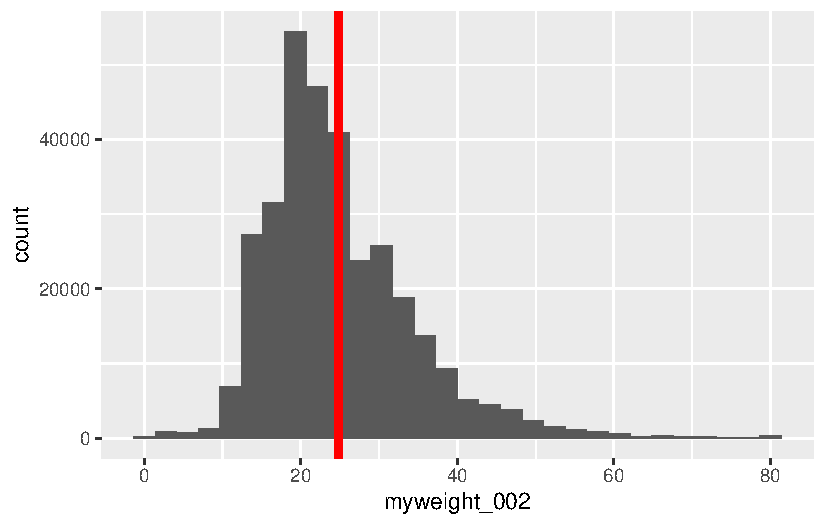
\includegraphics{BMI_help_files/figure-pdf/unnamed-chunk-8-1.pdf}

  }

  \end{figure}
\end{enumerate}

We need to convert the heights and weights to their cm and kg
respectively. Since I only have a number category, I've gone into the
codebook to find what each numbered category represents. If you put 8,
you are 43 inches tall; 16:51 in; and 32:67in. Now I can use a line to
see if I can create an equation to convert these values.

\[
\begin{align}
in & = m\times cat+b \\
43 &= m \times 8 + b \\
b & = 43-8m \\
\\
51 &= 16m + b \\
51 &= 16m + (43-8m) \\
m &=1 \\ 
b&=43-8m = 43-8=35 \\
\end{align}
\]

Then we double check with third set of points:

\[
\begin{align}
67 & = 1 \times 32 + 35 \\
67 & = 67 \\
\end{align}
\]

\begin{Shaded}
\begin{Highlighting}[]
\NormalTok{iat\_prep}\SpecialCharTok{$}\NormalTok{myheight\_in }\OtherTok{=} \DecValTok{1}\SpecialCharTok{*}\NormalTok{iat\_prep}\SpecialCharTok{$}\NormalTok{myheight\_002 }\SpecialCharTok{+} \DecValTok{35}
\end{Highlighting}
\end{Shaded}

Then we need to convert height to meters since BMI is in \(kg/m^2\).

\begin{Shaded}
\begin{Highlighting}[]
\NormalTok{iat\_prep}\SpecialCharTok{$}\NormalTok{myheight\_m }\OtherTok{=} \FloatTok{0.0254}\SpecialCharTok{*}\NormalTok{iat\_prep}\SpecialCharTok{$}\NormalTok{myheight\_in}
\end{Highlighting}
\end{Shaded}

Okay, now we need to do something similar for weight. Three more points
to find the conversion: 10:90lb; 20:140lb; and 30: 190lb.

\[
\begin{align}
lb & = m\times cat+b \\
90 &= m \times 10 + b \\
b & = 90-10m \\
\\
140 &= 20m + b \\
140 &= 20m + (90-10m) \\
m &=5 \\ 
b&=90-10m = 90-50=40 \\
\end{align}
\]

Then we double check with third set of points:

\[
\begin{align}
190 & = 5 \times 30 + 40 \\
190 & = 190 \\
\end{align}
\]

\begin{Shaded}
\begin{Highlighting}[]
\NormalTok{iat\_prep}\SpecialCharTok{$}\NormalTok{myweight\_lb }\OtherTok{=} \DecValTok{5}\SpecialCharTok{*}\NormalTok{iat\_prep}\SpecialCharTok{$}\NormalTok{myweight\_002 }\SpecialCharTok{+} \DecValTok{40}
\end{Highlighting}
\end{Shaded}

Then we need to convert height to meters since BMI is in \(kg/m^2\).

\begin{Shaded}
\begin{Highlighting}[]
\NormalTok{iat\_prep}\SpecialCharTok{$}\NormalTok{myweight\_kg }\OtherTok{=} \FloatTok{0.453592}\SpecialCharTok{*}\NormalTok{iat\_prep}\SpecialCharTok{$}\NormalTok{myweight\_lb}
\end{Highlighting}
\end{Shaded}

\begin{Shaded}
\begin{Highlighting}[]
\NormalTok{iat\_prep}\SpecialCharTok{$}\NormalTok{bmi }\OtherTok{=}\NormalTok{ iat\_prep}\SpecialCharTok{$}\NormalTok{myweight\_kg}\SpecialCharTok{/}\NormalTok{(iat\_prep}\SpecialCharTok{$}\NormalTok{myheight\_m)}\SpecialCharTok{\^{}}\DecValTok{2}
\end{Highlighting}
\end{Shaded}

\begin{Shaded}
\begin{Highlighting}[]
\FunctionTok{ggplot}\NormalTok{(}\AttributeTok{data =}\NormalTok{ iat\_prep, }\FunctionTok{aes}\NormalTok{(}\AttributeTok{x =}\NormalTok{ bmi)) }\SpecialCharTok{+} 
  \FunctionTok{geom\_histogram}\NormalTok{(}\AttributeTok{binwidth =} \DecValTok{1}\NormalTok{) }\SpecialCharTok{+}
  \FunctionTok{geom\_vline}\NormalTok{(}\FunctionTok{aes}\NormalTok{(}\AttributeTok{xintercept =} \FunctionTok{mean}\NormalTok{(bmi, }
                                   \AttributeTok{na.rm =}\NormalTok{ T)), }
             \AttributeTok{color =} \StringTok{"red"}\NormalTok{, }\AttributeTok{linewidth =} \DecValTok{2}\NormalTok{)}
\end{Highlighting}
\end{Shaded}

\begin{verbatim}
Warning: Removed 142470 rows containing non-finite outside the scale range
(`stat_bin()`).
\end{verbatim}

\begin{figure}[H]

{\centering 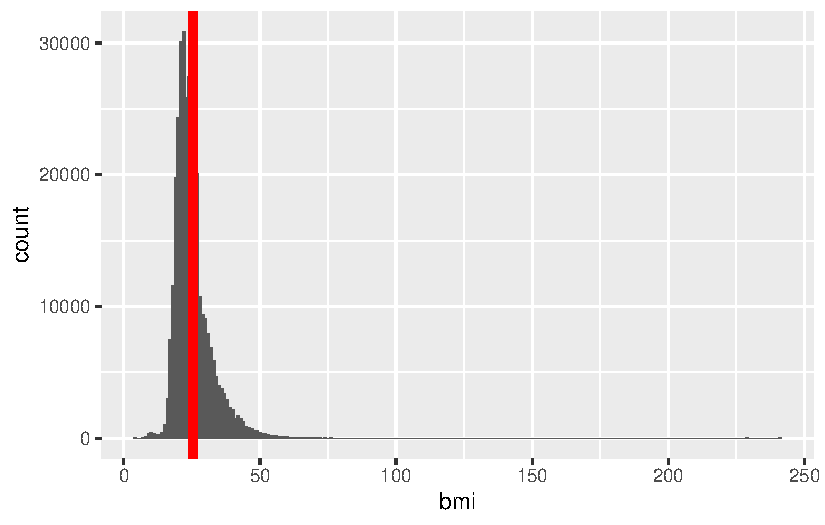
\includegraphics{BMI_help_files/figure-pdf/unnamed-chunk-14-1.pdf}

}

\end{figure}

From histogram, looks like there are a couple observations at BMIs
greater than 200. Let's double check that.

\begin{Shaded}
\begin{Highlighting}[]
\FunctionTok{summary}\NormalTok{(iat\_prep}\SpecialCharTok{$}\NormalTok{bmi)}
\end{Highlighting}
\end{Shaded}

\begin{verbatim}
   Min. 1st Qu.  Median    Mean 3rd Qu.    Max.    NA's 
   4.28   20.81   23.71   25.48   28.21  241.41  142470 
\end{verbatim}

Okay, so we now know the max is 241.41. I want to see the observations
that have BMIs this large. I'll take a look at their other values to see
if there are any other issues.

\begin{Shaded}
\begin{Highlighting}[]
\NormalTok{iat\_prep\_bmi }\OtherTok{=}\NormalTok{ iat\_prep }\SpecialCharTok{\%\textgreater{}\%} \FunctionTok{filter}\NormalTok{(bmi }\SpecialCharTok{\textgreater{}} \DecValTok{200}\NormalTok{)}
\FunctionTok{head}\NormalTok{(iat\_prep\_bmi, }\DecValTok{10}\NormalTok{)}
\end{Highlighting}
\end{Shaded}

\begin{verbatim}
     IAT_score att7 iam_001 identfat_001 myweight_002 myheight_002
1  -0.61544208    4       1            5           81            2
2   0.54476890    1       6            2           80            1
3   0.70458996    1       2            3           80            2
4   0.28206698    6       7            1           81            1
5   0.33790313    5       7            3           81            2
6   1.23311171    1       7            4           80            2
7  -0.02357343    7       1            1           81            2
8           NA    7       1            1           81            2
9   0.33704837    4       1            1           81            2
10 -0.47687442    4       4           NA           81            1
   identthin_001 controlother_001 controlyou_001 mostpref_001 important_001
1              1                5              5            4             5
2              3                4              4            3             1
3              3                3              2            4             5
4              5                1              1            6             5
5              4                3              2            1             4
6              1                5              1            1             2
7              5                1              1            2             5
8              5                1              5            7             5
9              5                1              1            4             4
10            NA               NA              1           NA            NA
   birthmonth birthyear month year raceomb_002    raceombmulti ethnicityomb edu
1          12      1910     1 2021           8 [1,2,3,4,5,6,7]            1  12
2          12      2009     1 2021           4                            1   1
3          10      1916     1 2021           4                            1   1
4          11      1910     2 2021          NA                            3   1
5           4      2007     2 2021           6                            3  NA
6           5      2001     2 2021           6                            2   5
7           2      1980     2 2021           8 [1,2,3,4,5,6,7]            1   9
8          NA        NA     2 2021          NA                           NA  NA
9           5      1976     2 2021           5                            2   4
10          9        NA     2 2021        -999                           NA  NA
   edu_14 genderIdentity birthSex myheight_in myheight_m myweight_lb
1      12            [2]        2          37     0.9398         445
2       1            [1]        1          36     0.9144         440
3       1            [1]        1          37     0.9398         440
4       1            [6]        2          36     0.9144         445
5      NA            [1]        1          37     0.9398         445
6       5            [1]        1          37     0.9398         440
7       9  [1,2,3,4,5,6]        2          37     0.9398         445
8      NA                      NA          37     0.9398         445
9       4            [1]        1          37     0.9398         445
10     NA            [2]        2          36     0.9144         445
   myweight_kg      bmi
1     201.8484 228.5359
2     199.5805 238.6963
3     199.5805 225.9681
4     201.8484 241.4087
5     201.8484 228.5359
6     199.5805 225.9681
7     201.8484 228.5359
8     201.8484 228.5359
9     201.8484 228.5359
10    201.8484 241.4087
\end{verbatim}

Looking at the subset of individuals with BMIs greater than 200, I am
reminded that there is some serious quality control that needs to be
done to this dataset. Other variable observations indicate that some of
these rows are individuals who did not accurately fill out their survey.
Right now, we keep them in our dataset, but we will need to examine them
for outliers.



\end{document}
